\subsection{Test Setup}
In order to properly validate our implementation, we tested our design using a test-bench; this test-bench can generate random numbers, compute the results of our implementation and then compare them with the results of the C function \emph{sqrtf} (that can be found in \emph{math.h}).  \\
All the other functions and operations already developed for the FPU were tested this way, so we extended two existing files:
\begin{itemize}
\item dpi\_lampFPU.c is a C file; we added the functions \emph{DPI\_sqrt} and \emph{DPI\_invSqrt}. Given a value X, They return the value of $\sqrt{X}$ and $\frac{1}{\sqrt{X}}$, as unsigned integer representing a number in binary32.
\item tb\_lampFPU.sv is a SystemVerilog file; it instantiates the FPU, imports the C functions and compares their results with the ones produced by the top module. 
\end{itemize}

In order to test our implementation, we added two different tasks:
\begin{itemize}
\item \emph{TASK\_doSqrt\_op} takes as input the number X we want the square root of, calls the right C function defined in dpi\_lampFPU.c depending on the opcode, and saves the result. Then, the task rounds this result and compute $\sqrt{X}$ or $\frac{1}{\sqrt{X}}$ using our implementation. Then, the two results are compared. If they're the same, the test is passed, otherwise it fails. 
\item \emph{TASK\_testSqrt} creates a loop with 5000 iterations; in each one, it randomly generates values for the sign, the exponent and the mantissa, and calls \emph{TASK\_doSqrt\_op}. It also manages all the special cases, explicitly creating a test for each of them. 
\end{itemize}

\subsection{Results}
We ran our test-bench using the Vivado software, performing a behavioural, post-synthesis and post-implementation simulation. The results in all three cases are the same, and completely validate our implementation; out of 5000 tests performed, we're able to correctly compute the square root of all of them, obtaining zero rejections. \\
For the inverse square root, instead, we have a very small set of tests rejected for the behavioural simulation (21 out of 5000, the 0,42\%); in all these cases, our implementation returns the right exponent and sign, but has a mantissa one bit greater than expected. The issue possibly lies in the rounding function.  

\subsection{Algorithm Simulation}
In this section we show the efficiency of the algorithm for one randomly selected value. In order to keep the description as simple as possible, we will focus only on some signals and their values.\\ 
In the following pictures, the colour red is reserved to the clock and reset signals, the light blue to the module lampFPU\_sqrt.sv and the green to the module lampFPU\_fractSqrt.sv \\
\begin{figure}[h]
	\centering
	\captionsetup{justification=centering}
	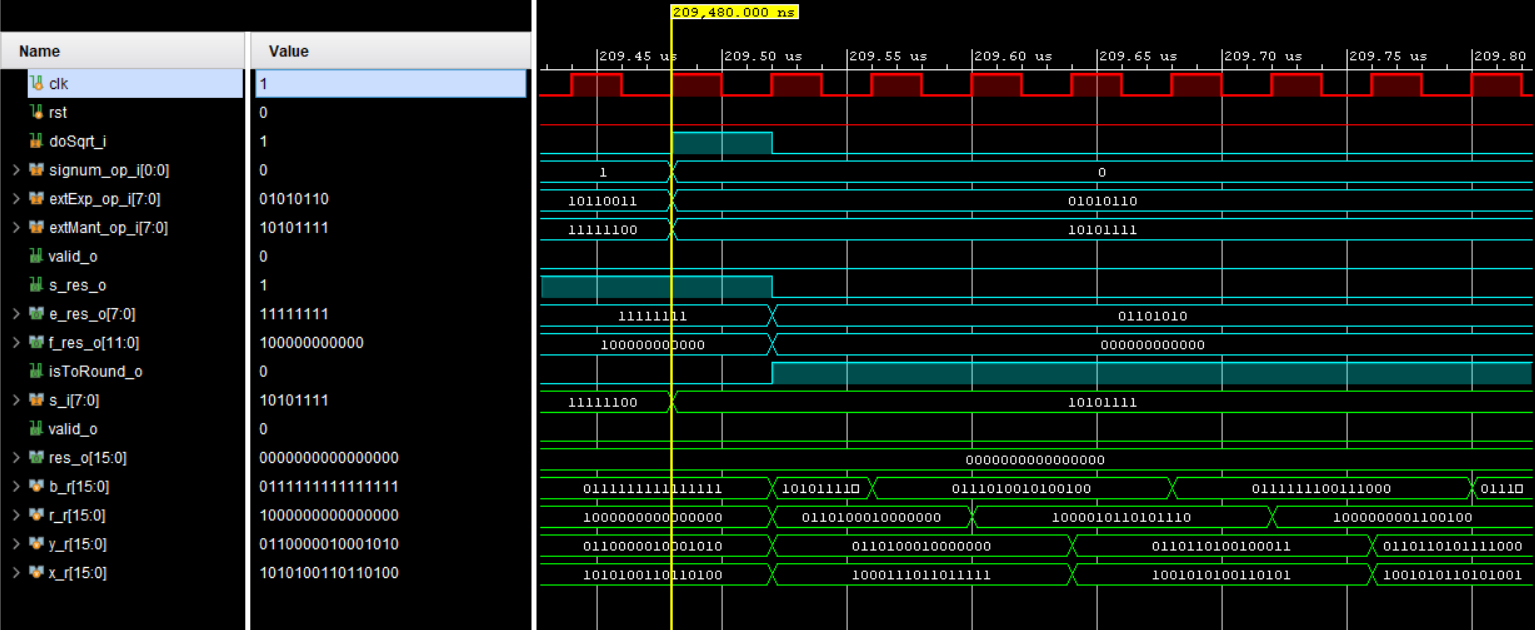
\includegraphics[width=\linewidth]{Simulation0.png}	
	\caption{First part of the simulation}
\end{figure}

\begin{itemize}
\item The test start at time 209.48 $\mu$s, when the signal doSqrt\_i is set to 1. We can see from the blue signals just under doSqrt\_i that the input number is positive, has exponent 01010110 (-41) and mantissa 10101111, so is the decimal number $6.217249*10^{-13}$; the mantissa, considered without the exponent, is the decimal number 1.3671875. We need a clock cycle before this information is propagated to the inner module, lampFPU\_fractSqrt.sv (green signals), which still has some values left from the previous test. We remember that for each internal signal shown in this simulation (for example b\_r) there is another one (b\_r\_next), not visualized for clarity.
\item In the next clock cycle (209.52 $\mu$s), lampFPU\_sqrt.sv recognizes we're not in a special case, so it computes the final exponent and sets \emph{isToRound\_o} to 1. Now, this module will wait until the inner one finishes its task.\\
In lampFPU\_fractSqrt.sv, all the internal registers are initialized. We refer to Section \ref{goldschmidt} for a complete description of the algorithm; since it's the first iteration, $B_0$ is set to the extended mantissa input and $Y_0$ is equal to $R_0$. 
\item In the next clock cycles we can see the evolution of the algorithm; depending on the current state, we update b\_r, r\_r, or y\_r and x\_r. To note, r\_r from the first to the second cycle becomes grater than 1, but then it keeps decreasing.
\item After only 10 clock cycles, r\_r becomes exactly 1; we need two more clock cycles in order to propagate the computed result. We can see that: 
$$x_r = 1001010110101001$$However, the input exponent is odd ($01010110$, or $-41$), so we need to multiply
$x_r * \sqrt{2}$. At time $209.92 \mu$s the inner module sets \emph{valid\_o} to 1 and gives us the final result, that is $1101001110100110$, or $1.6535034$ The Windows calculator instead computes $1.65359457$. 
\item This result is passed to the outer module, that returns it to lampFPU\_top.sv, puts the overflow bit to 0, computes the sticky bit and sets \emph{valid\_o} to 1. The 12 bits now are:
$$f\_res\_o = 011010011101$$ 
\item The top module now rounds the results (not shown in the diagram); using the rounding rules described in Section \ref{design}, we obtain the final value of the mantissa:
$$ M = (1)1010100 = 1.65625$$
This value is a bit greater than the real one but we have to remember that we only have 8 bits of precision; indeed, the value rounded down instead of up would be:
 $$ M' = (1)1010011 =1.6484375$$
The difference between M' and the real value is greater than the difference between M and the real one.
\item The test finishes and prints the results (fig.\ref{simRes}). We can see that it passes the test. 
\end{itemize}
\begin{figure}[h]
	\centering
	\captionsetup{justification=centering}
	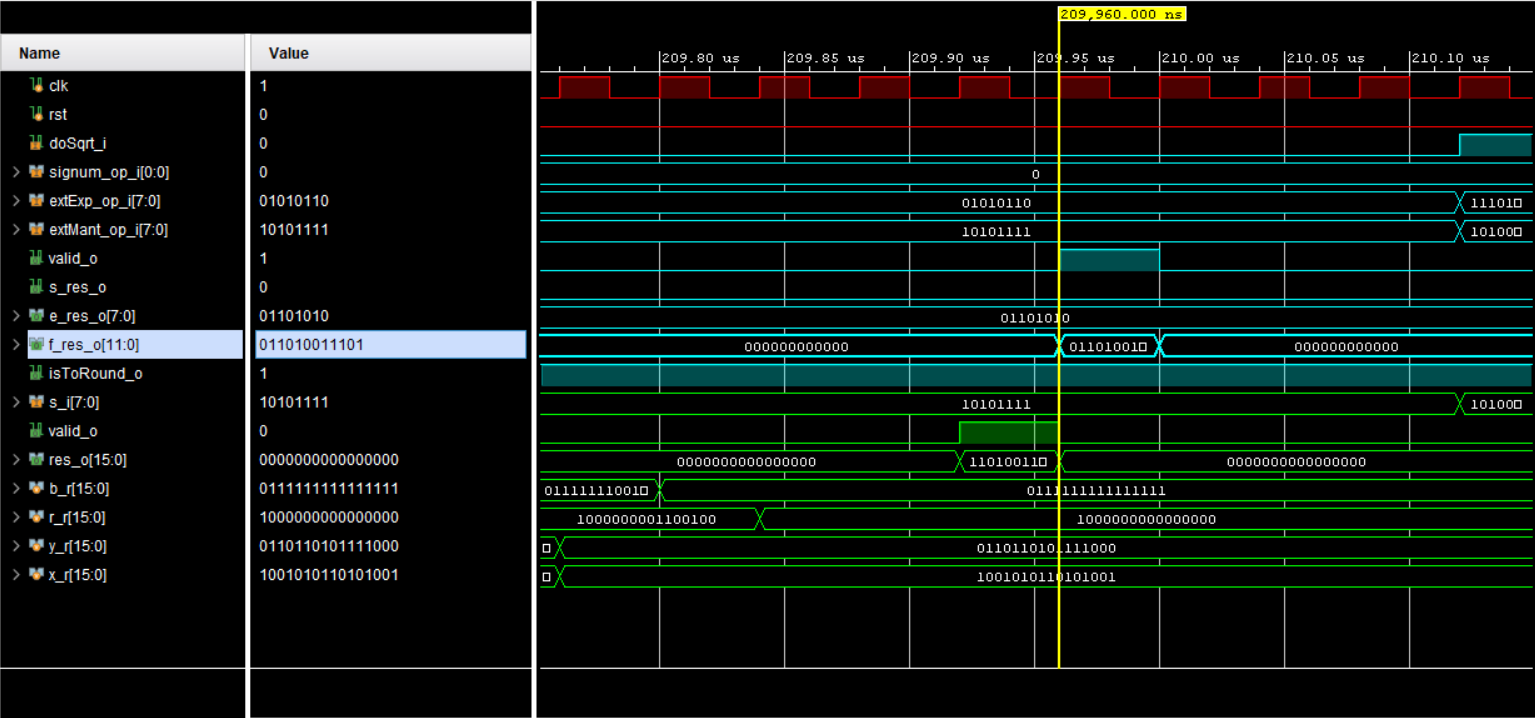
\includegraphics[width=\linewidth]{Simulation1.png}	
	\caption{Second part of the simulation}
\end{figure}
\begin{figure}[h]
	\centering
	\captionsetup{justification=centering}
	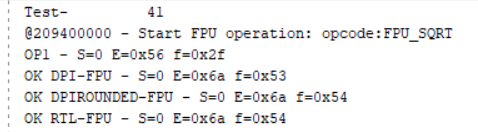
\includegraphics[width=\linewidth]{SimulationResult.png}	
	\caption{Final results of the simulation}
	\label{simRes}
\end{figure}


\subsection{Timing Results}
As shown in the algorithm simulation, we're able to properly compute, round and manage our results in only 12 clock cycles. We firstly used the frequency already set in the test-bench module (one clock cycle every 40 ns), but then we tried to lower this value in order to check how fast our modules could operate. We found out that our implementation can still work using a way smaller clock frequency (clock period of 6 ns, more than 6 times faster). 
\clearpage